\documentclass[11pt]{article}
\usepackage[T1]{fontenc}
\usepackage{graphicx,amsmath,amssymb}
\usepackage[margin=23mm]{geometry}
\usepackage{booktabs,longtable,array}
\usepackage[super,sort&compress]{natbib}
\usepackage[hidelinks]{hyperref}
\usepackage{setspace}
\onehalfspacing
\raggedright
\setlength{\parindent}{0pt}
\setlength{\parskip}{5pt}
\begin{document}
\title{Supplementary Information\\[6pt]\large Bayesian inference of target-associated migration changes in synthetic killer-cell trajectories}
\author{}
\date{}
\maketitle
\begin{center}Computational manuscript draft. All results are synthetic.\end{center}
\tableofcontents
\clearpage
\section{Scope and reproducibility record}
This supplement contains mathematical derivations, full numerical comparisons and diagnostic figures for a synthetic study of proximity-associated motility. It is intended to make the distinction between numerical correctness, parameter recovery, detection and mechanism attribution explicit. No experimental observations, biological replicates, clinical records or human-subject data were analyzed. ``Killer'' and ``target'' identify roles within the simulator; their geometry and parameter values are controlled benchmark choices.

The initial results in \texttt{results/synthetic\_v1} are retained as an exploratory stage. The follow-up results in \texttt{results/manuscript\_v2} were generated from plans written before the additional computations, with separate seed ranges. Those plans followed inspection of the initial results and do not constitute a preregistration. The expanded calibration and decision ensembles were evaluated using frozen numerical thresholds. Neural networks were not selected using scientific test performance. First training seeds were designated primary, and all remaining seeds are reported as sensitivity analyses.

A simulated movie is the independent unit for evaluation. Its 12 cells share geometry and generating global parameters; its successive frames have temporal dependence. Neither the number of frames nor the number of cells is used as the denominator of calibration or declaration rates. Several neural networks evaluate the same movies. Their outputs are reported separately rather than concatenated into a larger apparent sample.

The supplied source snapshot includes parameter priors, observation settings, random-seed partitions, inference scripts, plotting scripts and manuscript templates. The expanded neural experiments generated 24,000 training movies and 4,048 evaluation movies, including 336 movies matched to the state-space study. Regenerating those matched movies for state-space fitting does not create 336 additional independent evaluation datasets. Source hashes permit the state-space and neural comparisons to be checked at the observed-position level.

\section{Integrated Ornstein--Uhlenbeck transition}
\subsection{Joint velocity and position innovations}
For one spatial coordinate, hold $S$, $\tau$ and $J$ constant over interval $h$. With initial velocity $v_0$, the Ornstein--Uhlenbeck solution is
\begin{equation}
 v_h=e^{-h/\tau}v_0+\sqrt{2S^2/\tau}\int_0^h e^{-(h-s)/\tau}\,dW_v(s).
\end{equation}
Integrating velocity gives
\begin{equation}
 x_h-x_0=\tau(1-e^{-h/\tau})v_0+\sqrt{2S^2\tau}\int_0^h[1-e^{-(h-s)/\tau}]\,dW_v(s)+J\int_0^h dW_x(s).
\end{equation}
The same velocity-driving Brownian process appears in both equations. Its contributions are therefore correlated. Ito isometry yields the covariance entries in the main Methods:
\begin{align}
 Q_{vv}&=S^2(1-e^{-2h/\tau}),\\
 Q_{vx}&=S^2\tau(1-e^{-h/\tau})^2,\\
 Q_{xx}&=S^2\tau^2[2h/\tau-4(1-e^{-h/\tau})+(1-e^{-2h/\tau})]+J^2h.
\end{align}
Sampling the two innovations independently would discard $Q_{vx}$ and alter the relationship between displacement and subsequent velocity. The simulator instead samples their joint Gaussian distribution. The likelihood uses the same covariance identity, while independent unit tests compare it with matrix-exponential and covariance-integration calculations.

This transition is exact only conditional on constant coefficients within the step. The simulator evaluates proximity at the beginning of each internal step. It therefore approximates a spatially varying diffusion by locally frozen coefficients. Increasing internal substeps can change the distribution of target exposure and mechanical forces even though no Euler error is present in a constant-coefficient Ornstein--Uhlenbeck transition. The timestep experiment evaluates that separate source of numerical approximation.

\subsection{Stable evaluation at small intervals}
Let $a=h/\tau$. The difference $1-e^{-a}$ is evaluated using \texttt{expm1} to reduce cancellation. The bracket in $Q_{xx}$ has leading term $2a^3/3$ and becomes poorly conditioned if computed by subtracting nearly equal terms at very small $a$. The implementation switches to a local series in that regime. The velocity variance is non-negative, and the conditional position-innovation variance used in the Cholesky factor is protected against tiny negative roundoff. These numerical safeguards do not modify the intended finite covariance formula. They were checked against independent reference calculations over representative parameter and interval ranges.

\subsection{Locally stationary displacement statistics}
When velocity is stationary with variance $S^2$ and coefficients are constant, the integrated active displacement has variance
\begin{equation}
 V_A(h)=2S^2\tau[h-\tau(1-e^{-h/\tau})].
\end{equation}
Brownian displacement adds $V_J(h)=J^2h$, and independent localization errors at the two endpoints add $V_E=2\sigma_{\rm obs}^2$. Thus, the per-axis displacement variance is $V_A+V_J+V_E$. Its short-interval expansion is
\begin{equation}
 V_A(h)=S^2h^2-\frac{S^2}{3\tau}h^3+\frac{S^2}{12\tau^2}h^4+O(h^5).
\end{equation}
For non-overlapping increments separated by $k\geq1$ recording intervals, the active covariance is
\begin{equation}
 C_A(k)=S^2\tau^2(1-e^{-h/\tau})^2e^{-(k-1)h/\tau}.
\end{equation}
Brownian position increments do not contribute to this covariance. Differenced localization errors contribute $-\sigma_{\rm obs}^2$ at lag one and zero at larger lags. These expressions show why short-lag variability, localization noise and temporal memory must be modeled together. They also show why a large displacement variance alone is insufficient to identify persistence.

At $h=0.25$\,min, $\sigma_{\rm obs}=0.15\,\mu$m and zero cell offset, the far-field parameters $(3.2,1.6,0.7)$ give per-axis contributions of approximately 0.608, 0.1225 and 0.045\,$\mu$m$^2$ from active motion, jitter and localization, respectively. Under the strong combined contact response, the contributions are approximately 0.115, 0.607 and 0.045\,$\mu$m$^2$. The jitter fractions are therefore approximately 16\% and 79\%. Supplementary Fig.~S8 evaluates the same identities across recording intervals. This calculation is a local, stationary illustration. It does not assume that a cell crossing a distance gradient has already equilibrated to every instantaneous coefficient value.

The translational diffusion coefficient in the convention $dx=\sqrt{2D}\,dW$ is $D=J^2/2$. A 2.23-fold increase in $J$ is therefore approximately a 4.95-fold increase in $D$. All manuscript effect ratios for jitter refer to $J$, not to $D$. Similarly, $S$ is a stationary per-coordinate velocity standard deviation rather than mean scalar speed.

\section{Hierarchical likelihood and numerical posterior}
\subsection{Observation conditioning}
The Kalman filter marginalizes position and velocity for each cell and coordinate. Its initial true-position uncertainty is $\sigma_{\rm obs}^2$ after conditioning on the first recorded position under a flat initial-position prior. The initial velocity is zero-mean with local stationary variance. The likelihood sums innovation log densities after that first observation. Missing observations may be skipped, but their distance gates require interpolation in the current implementation; the main reported ensembles contain no missing positions.

The distance gate is computed from recorded killer positions. Consequently, the likelihood is a conditional approximation to the spatial simulator when localization error is present. It does not integrate over uncertainty in the covariate itself. The targets are treated as exactly known, and no observation likelihood for target segmentation or position is included. A future mask-based analysis would require an explicit distance operator, boundary treatment and uncertainty model. Applying this benchmark directly to unknown three-dimensional contact geometry would change its scientific meaning.

\subsection{Exact conditional hierarchy refresh}
The hierarchy is $b_i=\mu_S+u_i$, with independent $u_i\sim N(0,\sigma_u^2)$ and fixed $\sigma_u=0.25$. When the cell baselines $b_i$ are held fixed, the movement likelihood is unchanged by shifting $\mu_S$ and compensating each $u_i$. The conditional posterior for $\mu_S$ is a normal distribution with mean $\bar b$ and standard deviation $\sigma_u/\sqrt{N}$, truncated to the uniform-prior support of $\mu_S$. Sampling this conditional distribution and setting $u_i=b_i-\mu_S$ gives an exact Gibbs refresh. It improves movement along the population/intercept correlation without replacing the posterior by a Gaussian approximation.

The finite-difference Hessian at the optimized posterior mode only shapes Metropolis proposals. The independence proposal is a multivariate Student-$t$ distribution, and its forward/reverse density ratio is included in acceptance. Adaptation of the random-walk covariance and scale stops after warm-up. Independent random-number streams initialize and drive the four chains. Stored rank-normalized convergence and effective-sample diagnostics include all six global parameters and all 12 cell intercepts.

\subsection{Retries and unresolved fits}
The expanded state-space plan initially requests 2,000 retained draws per chain after 1,500 warm-up iterations. Subsequent attempts use 4,000 draws with 2,000 warm-up iterations, then 8,000, 16,000 or 32,000 draws with 3,000 warm-up iterations. The same prespecified criteria apply to every attempt: maximum rank-normalized $\widehat R<1.01$, minimum bulk effective sample size at least 400 and minimum tail effective sample size at least 400. Earlier attempt diagnostics and cumulative time remain in the records. Retries are triggered by numerical diagnostics, never by whether an estimated effect agrees with truth.

For any unresolved fits, primary rates are conditional on accepted fits, accompanied by attempted/accepted/failed counts and worst/best outcome bounds over all attempts. When all fits pass, these bounds coincide with ordinary rates. Passing this numerical gate does not establish model validity or guarantee that every posterior approximation is free of bias. The final counts and diagnostic distributions are given in Supplementary Table~S2 and Supplementary Fig.~S7.

\section{Neural context, training and usage}
\subsection{Summary construction and density transformation}
Each simulation contributes one row of 82 summaries derived only from observed killer tracks, observed target positions and acquisition settings. The vector describes multiscale increments, correlations, turning, radial movement, distance exposure, dwell and within-cell contrasts. It is not a sufficient statistic by proof. Summary compression may explain part of the neural persistence gap, and the present study does not compare all possible summary or sequence architectures.

Each bounded parameter $\theta_j\in(L_j,U_j)$ is mapped to $z_j=\operatorname{logit}[(\theta_j-L_j)/(U_j-L_j)]$ and standardized. A conditional mixture of three full-covariance Gaussian densities estimates the joint density in transformed space. Samples map back through the logistic transformation and remain inside prior support. Evaluating density in original parameter coordinates includes the corresponding Jacobian. Full Cholesky covariance matrices permit correlated parameter uncertainty; marginal coverage checks do not establish that these correlations are accurately calibrated.

Training uses a 15\% internal validation split at the movie level, AdamW optimization with learning rate 0.0015 and weight decay $10^{-4}$, batch size 128, gradient clipping at norm 5, at most 300 epochs and early-stopping patience 40. The best internal-validation checkpoint is restored. Input standardization uses training rows only. Standardized inputs are clipped to $[-12,12]$ inside the network for numerical stability, and Cholesky diagonal terms use softplus plus 0.025. These stabilizers are implementation choices, not safeguards against scientific extrapolation. All scientific evaluation movies are disjoint from the simulation banks and internal validation splits.

\subsection{Noise conditioning and ablation}
The fixed-protocol estimator expects 82 summaries. The noise-conditioned extension expects 83 context values: the same observed summaries followed by $\log\sigma_{\rm obs}$. The noise-marginalized extension uses 82 inputs but a broader training bank. The identical expanded bank supports the conditioned/marginalized comparison. The two models represent different conditional questions: the former uses a supplied known acquisition noise, whereas the latter averages over its training distribution.

The new checkpoints are research artifacts accessed using the documented \texttt{observed\_context} helper in the manuscript SBI script. They are not interchangeable with the original application wrapper, which checks an 82-feature fixed protocol. Supplying 83 values to an 82-feature network is a shape error; silently omitting the scalar would ask a different inference question. The usage note in the source snapshot gives an executable example and lists the remaining fixed nuisance assumptions. No experimental-data adapter is claimed.

\subsection{Validation interpretation}
Calibration evaluates parameter draws across the stated prior, so it averages over easy and difficult regions. Separate null and alternative cases evaluate specific decision behavior. A posterior with correct marginal coverage may still be uninformative, conditionally miscalibrated or wrong in its joint dependence. Therefore, interval widths, root-mean-squared errors, rank diagnostics and decision rates are reported together. Rank-histogram bands are pointwise binomial reference intervals, not simultaneous envelopes or formal acceptance regions. Network samples are approximate posterior draws; no rank plot establishes exact inference.

The training-seed sensitivity experiment reuses a common bank and common test movies. It therefore contains dependence across model results. We give each seed's coverage and decisions separately and do not assign a confidence interval to the range across three seeds. The frozen original model provides a prospective evaluation of an existing checkpoint. Primary new seeds were chosen numerically before evaluation. The publication figures identify the specific checkpoint shown so that favorable and unfavorable outcomes cannot be mixed across networks.

\section{Mechanics, source transfer and predictive checks}
The reduced mechanics are deliberately simple. Overlap repulsion is proportional to the positive difference between contact distance and centroid distance. A stochastic bond can form within contact, break at its dissociation rate, or break when distance exceeds a capture radius. Bonded killers receive a radial adhesive drift. Reduced-model targets move independently and do not receive reciprocal forces. The supplied source model retains reciprocal mechanical effects, making it a structurally distinct transfer generator.

A mechanical-only trajectory can exhibit real retention or altered turning while its intrinsic stochastic coefficients remain target-independent. Calling that condition a ``null'' without qualification would be misleading. Its ground truth is zero direct modulation of the intrinsic coefficients. Poor coverage or positive coefficient declarations assess attribution within a model that omits mechanics. They do not negate the physical change in the path.

The original mechanical benchmark used four internal steps per recorded frame. Supplementary Fig.~S5 compares this with finer settings and shows residual sensitivity in turning. Mechanical decision rates are therefore exploratory. Eight to sixteen internal steps provide a starting point for subsequent studies, but their apparent agreement in a finite ensemble is not a proof of convergence. Different stiffness, adhesion or density settings could require smaller timesteps.

Posterior predictive checks use the fitted baseline simulator, even when the observed movie came from a mechanical stress case. They condition on the observed starting positions and target geometry but redraw cell offsets from the population. One hundred predictive movies are generated per example/method. The 82 features are correlated and were used to construct or assess inference, so the fraction outside pointwise 90\% intervals is descriptive. The low discrepancy in the mechanical example demonstrates that acceptable predictive summaries may coexist with incorrect mechanism attribution (Supplementary Fig.~S6).

\section{Complete numerical tables}
All intervals in the following tables are two-sided 95\% Wilson Monte Carlo intervals unless explicitly described otherwise. Percentages are rounded for display; machine-readable source records retain full precision. ``Accepted'' refers only to the MCMC numerical gate. Neural tables report all independently generated evaluation movies. No table pools the same movies across network seeds.

Network abbreviations are F0 (frozen original model), F1--F3 (new fixed-noise seeds 117001--117003), C1--C3 (noise-conditioned seeds 127001--127003) and M1--M3 (noise-marginalized models using those same seeds). Counts labeled $S/\tau/J$ are the separate directional declarations for the three proximity effects. Their sum need not equal the any-effect count, because a movie can receive more than one declaration.
\subsection*{Supplementary Table S1 | Expanded sampling counts}
\small
\begin{longtable}{>{\raggedright\arraybackslash}p{0.215\textwidth}>{\raggedright\arraybackslash}p{0.215\textwidth}>{\raggedright\arraybackslash}p{0.215\textwidth}>{\raggedright\arraybackslash}p{0.215\textwidth}}
\toprule
Ensemble & Planned & Accepted & Unresolved \\
\midrule
\endfirsthead
\toprule
Ensemble & Planned & Accepted & Unresolved \\
\midrule
\endhead
Calibration & 96 & 96 & 0 \\
Fixed null & 96 & 96 & 0 \\
Combined & 96 & 96 & 0 \\
Varied-baseline null & 48 & 48 & 0 \\
\bottomrule
\end{longtable}
\normalsize

\subsection*{Supplementary Table S2 | State-space calibration}
\small
\begin{longtable}{>{\raggedright\arraybackslash}p{0.215\textwidth}>{\raggedright\arraybackslash}p{0.215\textwidth}>{\raggedright\arraybackslash}p{0.215\textwidth}>{\raggedright\arraybackslash}p{0.215\textwidth}}
\toprule
Parameter & 90\% coverage [interval] & RMSE & Mean 90\% width \\
\midrule
\endfirsthead
\toprule
Parameter & 90\% coverage [interval] & RMSE & Mean 90\% width \\
\midrule
\endhead
$\mu_S$ & 94.8\% [88.4\%, 97.8\%] & 0.062 & 0.242 \\
$\mu_\tau$ & 89.6\% [81.9\%, 94.2\%] & 0.108 & 0.357 \\
$\mu_J$ & 93.8\% [87.0\%, 97.1\%] & 0.045 & 0.148 \\
$\delta_S$ & 91.7\% [84.4\%, 95.7\%] & 0.109 & 0.331 \\
$\delta_\tau$ & 89.6\% [81.9\%, 94.2\%] & 0.258 & 0.716 \\
$\delta_J$ & 93.8\% [87.0\%, 97.1\%] & 0.082 & 0.273 \\
\bottomrule
\end{longtable}
\normalsize

\subsection*{Supplementary Table S3 | Neural calibration by seed}
\small
\begin{longtable}{>{\raggedright\arraybackslash}p{0.215\textwidth}>{\raggedright\arraybackslash}p{0.215\textwidth}>{\raggedright\arraybackslash}p{0.215\textwidth}>{\raggedright\arraybackslash}p{0.215\textwidth}}
\toprule
Network & Parameter & 90\% coverage [interval] & RMSE \\
\midrule
\endfirsthead
\toprule
Network & Parameter & 90\% coverage [interval] & RMSE \\
\midrule
\endhead
F0 & $\mu_S$ & 91.0\% [89.1\%, 92.6\%] & 0.094 \\
F0 & $\mu_\tau$ & 92.9\% [91.1\%, 94.3\%] & 0.135 \\
F0 & $\mu_J$ & 92.2\% [90.4\%, 93.7\%] & 0.060 \\
F0 & $\delta_S$ & 89.6\% [87.6\%, 91.4\%] & 0.159 \\
F0 & $\delta_\tau$ & 91.9\% [90.1\%, 93.4\%] & 0.279 \\
F0 & $\delta_J$ & 92.7\% [90.9\%, 94.1\%] & 0.118 \\
F1 & $\mu_S$ & 91.2\% [89.3\%, 92.8\%] & 0.095 \\
F1 & $\mu_\tau$ & 91.6\% [89.7\%, 93.1\%] & 0.134 \\
F1 & $\mu_J$ & 89.9\% [87.9\%, 91.6\%] & 0.062 \\
F1 & $\delta_S$ & 90.5\% [88.6\%, 92.2\%] & 0.160 \\
F1 & $\delta_\tau$ & 90.7\% [88.8\%, 92.4\%] & 0.291 \\
F1 & $\delta_J$ & 91.0\% [89.1\%, 92.6\%] & 0.122 \\
F2 & $\mu_S$ & 91.6\% [89.7\%, 93.1\%] & 0.096 \\
F2 & $\mu_\tau$ & 91.9\% [90.1\%, 93.4\%] & 0.139 \\
F2 & $\mu_J$ & 92.4\% [90.6\%, 93.9\%] & 0.064 \\
F2 & $\delta_S$ & 91.9\% [90.1\%, 93.4\%] & 0.157 \\
F2 & $\delta_\tau$ & 93.1\% [91.3\%, 94.5\%] & 0.283 \\
F2 & $\delta_J$ & 91.8\% [90.0\%, 93.3\%] & 0.126 \\
F3 & $\mu_S$ & 90.6\% [88.7\%, 92.3\%] & 0.095 \\
F3 & $\mu_\tau$ & 91.9\% [90.1\%, 93.4\%] & 0.134 \\
F3 & $\mu_J$ & 92.0\% [90.2\%, 93.5\%] & 0.060 \\
F3 & $\delta_S$ & 89.3\% [87.2\%, 91.0\%] & 0.157 \\
F3 & $\delta_\tau$ & 92.6\% [90.8\%, 94.0\%] & 0.279 \\
F3 & $\delta_J$ & 89.9\% [87.9\%, 91.6\%] & 0.127 \\
\bottomrule
\end{longtable}
\normalsize

\subsection*{Supplementary Table S4 | Neural decisions by seed}
\small
\begin{longtable}{>{\raggedright\arraybackslash}p{0.172\textwidth}>{\raggedright\arraybackslash}p{0.172\textwidth}>{\raggedright\arraybackslash}p{0.172\textwidth}>{\raggedright\arraybackslash}p{0.172\textwidth}>{\raggedright\arraybackslash}p{0.172\textwidth}}
\toprule
Network & Scenario & Any / $n$ & 95\% interval & Counts $S/\tau/J$ \\
\midrule
\endfirsthead
\toprule
Network & Scenario & Any / $n$ & 95\% interval & Counts $S/\tau/J$ \\
\midrule
\endhead
F0 & null & 3/256 & [0.4\%, 3.4\%] & 1/1/1 \\
F0 & Varied null & 3/256 & [0.4\%, 3.4\%] & 1/2/0 \\
F0 & slowdown & 127/128 & [95.7\%, 99.9\%] & 127/0/0 \\
F0 & decorrelation & 45/128 & [27.4\%, 43.8\%] & 0/45/0 \\
F0 & jitter & 128/128 & [97.1\%, 100.0\%] & 0/0/128 \\
F0 & combined & 128/128 & [97.1\%, 100.0\%] & 119/5/128 \\
F0 & weak & 43/128 & [26.0\%, 42.1\%] & 23/3/28 \\
F1 & null & 2/256 & [0.2\%, 2.8\%] & 1/0/1 \\
F1 & Varied null & 1/256 & [0.1\%, 2.2\%] & 0/1/0 \\
F1 & slowdown & 124/128 & [92.2\%, 98.8\%] & 124/1/0 \\
F1 & decorrelation & 42/128 & [25.3\%, 41.3\%] & 0/42/0 \\
F1 & jitter & 128/128 & [97.1\%, 100.0\%] & 0/0/128 \\
F1 & combined & 128/128 & [97.1\%, 100.0\%] & 114/17/128 \\
F1 & weak & 45/128 & [27.4\%, 43.8\%] & 15/4/33 \\
F2 & null & 6/256 & [1.1\%, 5.0\%] & 1/4/1 \\
F2 & Varied null & 4/256 & [0.6\%, 3.9\%] & 1/3/0 \\
F2 & slowdown & 123/128 & [91.2\%, 98.3\%] & 123/0/0 \\
F2 & decorrelation & 61/128 & [39.2\%, 56.3\%] & 0/61/0 \\
F2 & jitter & 128/128 & [97.1\%, 100.0\%] & 0/0/128 \\
F2 & combined & 128/128 & [97.1\%, 100.0\%] & 114/17/128 \\
F2 & weak & 46/128 & [28.1\%, 44.5\%] & 21/6/30 \\
F3 & null & 4/256 & [0.6\%, 3.9\%] & 2/2/1 \\
F3 & Varied null & 3/256 & [0.4\%, 3.4\%] & 1/1/1 \\
F3 & slowdown & 127/128 & [95.7\%, 99.9\%] & 127/0/0 \\
F3 & decorrelation & 56/128 & [35.5\%, 52.4\%] & 0/56/0 \\
F3 & jitter & 128/128 & [97.1\%, 100.0\%] & 0/0/128 \\
F3 & combined & 128/128 & [97.1\%, 100.0\%] & 120/12/128 \\
F3 & weak & 59/128 & [37.7\%, 54.7\%] & 32/5/41 \\
\bottomrule
\end{longtable}
\normalsize

\subsection*{Supplementary Table S5 | Observation-noise decisions}
\small
\begin{longtable}{>{\raggedright\arraybackslash}p{0.172\textwidth}>{\raggedright\arraybackslash}p{0.172\textwidth}>{\raggedright\arraybackslash}p{0.172\textwidth}>{\raggedright\arraybackslash}p{0.172\textwidth}>{\raggedright\arraybackslash}p{0.172\textwidth}}
\toprule
Network & Scenario & Any / $n$ & 95\% interval & Counts $S/\tau/J$ \\
\midrule
\endfirsthead
\toprule
Network & Scenario & Any / $n$ & 95\% interval & Counts $S/\tau/J$ \\
\midrule
\endhead
F0 & Null 0.15 & 0/128 & [0.0\%, 2.9\%] & 0/0/0 \\
F0 & Null 0.60 & 128/128 & [97.1\%, 100.0\%] & 128/0/27 \\
F0 & Combined 0.15 & 128/128 & [97.1\%, 100.0\%] & 116/10/128 \\
F0 & Combined 0.60 & 128/128 & [97.1\%, 100.0\%] & 128/0/73 \\
C1 & Null 0.15 & 0/128 & [0.0\%, 2.9\%] & 0/0/0 \\
C1 & Null 0.60 & 1/128 & [0.1\%, 4.3\%] & 1/0/0 \\
C1 & Combined 0.15 & 128/128 & [97.1\%, 100.0\%] & 114/22/128 \\
C1 & Combined 0.60 & 123/128 & [91.2\%, 98.3\%] & 86/2/121 \\
C2 & Null 0.15 & 0/128 & [0.0\%, 2.9\%] & 0/0/0 \\
C2 & Null 0.60 & 1/128 & [0.1\%, 4.3\%] & 0/0/1 \\
C2 & Combined 0.15 & 128/128 & [97.1\%, 100.0\%] & 119/10/128 \\
C2 & Combined 0.60 & 124/128 & [92.2\%, 98.8\%] & 106/0/120 \\
C3 & Null 0.15 & 0/128 & [0.0\%, 2.9\%] & 0/0/0 \\
C3 & Null 0.60 & 2/128 & [0.4\%, 5.5\%] & 1/0/1 \\
C3 & Combined 0.15 & 128/128 & [97.1\%, 100.0\%] & 119/10/128 \\
C3 & Combined 0.60 & 123/128 & [91.2\%, 98.3\%] & 100/2/119 \\
M1 & Null 0.15 & 0/128 & [0.0\%, 2.9\%] & 0/0/0 \\
M1 & Null 0.60 & 3/128 & [0.8\%, 6.7\%] & 2/0/1 \\
M1 & Combined 0.15 & 128/128 & [97.1\%, 100.0\%] & 110/23/128 \\
M1 & Combined 0.60 & 121/128 & [89.1\%, 97.3\%] & 102/0/120 \\
M2 & Null 0.15 & 0/128 & [0.0\%, 2.9\%] & 0/0/0 \\
M2 & Null 0.60 & 1/128 & [0.1\%, 4.3\%] & 0/0/1 \\
M2 & Combined 0.15 & 128/128 & [97.1\%, 100.0\%] & 112/17/128 \\
M2 & Combined 0.60 & 119/128 & [87.2\%, 96.3\%] & 82/3/118 \\
M3 & Null 0.15 & 0/128 & [0.0\%, 2.9\%] & 0/0/0 \\
M3 & Null 0.60 & 1/128 & [0.1\%, 4.3\%] & 0/0/1 \\
M3 & Combined 0.15 & 128/128 & [97.1\%, 100.0\%] & 114/20/128 \\
M3 & Combined 0.60 & 118/128 & [86.2\%, 95.7\%] & 94/5/103 \\
\bottomrule
\end{longtable}
\normalsize

\subsection*{Supplementary Table S6 | Calibration across noise}
\small
\begin{longtable}{>{\raggedright\arraybackslash}p{0.172\textwidth}>{\raggedright\arraybackslash}p{0.172\textwidth}>{\raggedright\arraybackslash}p{0.172\textwidth}>{\raggedright\arraybackslash}p{0.172\textwidth}>{\raggedright\arraybackslash}p{0.172\textwidth}}
\toprule
Network & Parameter & 90\% coverage & RMSE & 90\% width \\
\midrule
\endfirsthead
\toprule
Network & Parameter & 90\% coverage & RMSE & 90\% width \\
\midrule
\endhead
F0 & $\mu_S$ & 76.3\% & 0.125 & 0.284 \\
F0 & $\mu_\tau$ & 86.2\% & 0.188 & 0.533 \\
F0 & $\mu_J$ & 54.9\% & 0.396 & 0.464 \\
F0 & $\delta_S$ & 70.8\% & 0.364 & 0.509 \\
F0 & $\delta_\tau$ & 87.4\% & 0.478 & 1.077 \\
F0 & $\delta_J$ & 72.7\% & 0.391 & 0.569 \\
C1 & $\mu_S$ & 91.7\% & 0.095 & 0.325 \\
C1 & $\mu_\tau$ & 92.4\% & 0.135 & 0.487 \\
C1 & $\mu_J$ & 90.1\% & 0.091 & 0.289 \\
C1 & $\delta_S$ & 92.4\% & 0.158 & 0.564 \\
C1 & $\delta_\tau$ & 89.9\% & 0.311 & 0.968 \\
C1 & $\delta_J$ & 91.5\% & 0.157 & 0.506 \\
C2 & $\mu_S$ & 92.4\% & 0.095 & 0.336 \\
C2 & $\mu_\tau$ & 91.8\% & 0.136 & 0.487 \\
C2 & $\mu_J$ & 91.9\% & 0.095 & 0.300 \\
C2 & $\delta_S$ & 93.3\% & 0.159 & 0.566 \\
C2 & $\delta_\tau$ & 91.4\% & 0.313 & 1.009 \\
C2 & $\delta_J$ & 92.4\% & 0.161 & 0.525 \\
C3 & $\mu_S$ & 90.9\% & 0.098 & 0.328 \\
C3 & $\mu_\tau$ & 92.5\% & 0.137 & 0.500 \\
C3 & $\mu_J$ & 89.9\% & 0.093 & 0.286 \\
C3 & $\delta_S$ & 93.1\% & 0.159 & 0.556 \\
C3 & $\delta_\tau$ & 91.3\% & 0.306 & 1.011 \\
C3 & $\delta_J$ & 91.1\% & 0.163 & 0.501 \\
M1 & $\mu_S$ & 92.4\% & 0.096 & 0.337 \\
M1 & $\mu_\tau$ & 92.0\% & 0.141 & 0.513 \\
M1 & $\mu_J$ & 92.7\% & 0.161 & 0.508 \\
M1 & $\delta_S$ & 93.9\% & 0.157 & 0.581 \\
M1 & $\delta_\tau$ & 92.0\% & 0.315 & 1.024 \\
M1 & $\delta_J$ & 92.1\% & 0.173 & 0.577 \\
M2 & $\mu_S$ & 92.6\% & 0.097 & 0.328 \\
M2 & $\mu_\tau$ & 92.5\% & 0.140 & 0.519 \\
M2 & $\mu_J$ & 92.2\% & 0.157 & 0.513 \\
M2 & $\delta_S$ & 94.0\% & 0.159 & 0.595 \\
M2 & $\delta_\tau$ & 90.8\% & 0.317 & 1.006 \\
M2 & $\delta_J$ & 92.7\% & 0.174 & 0.585 \\
M3 & $\mu_S$ & 91.5\% & 0.097 & 0.340 \\
M3 & $\mu_\tau$ & 93.1\% & 0.140 & 0.517 \\
M3 & $\mu_J$ & 92.9\% & 0.157 & 0.518 \\
M3 & $\delta_S$ & 91.3\% & 0.158 & 0.568 \\
M3 & $\delta_\tau$ & 91.9\% & 0.323 & 1.021 \\
M3 & $\delta_J$ & 92.8\% & 0.171 & 0.589 \\
\bottomrule
\end{longtable}
\normalsize

\subsection*{Supplementary Table S7 | Paired movie decisions}
\small
\begin{longtable}{>{\raggedright\arraybackslash}p{0.172\textwidth}>{\raggedright\arraybackslash}p{0.172\textwidth}>{\raggedright\arraybackslash}p{0.172\textwidth}>{\raggedright\arraybackslash}p{0.172\textwidth}>{\raggedright\arraybackslash}p{0.172\textwidth}}
\toprule
Method & Scenario & Any / $n$ & 95\% interval & Counts $S/\tau/J$ \\
\midrule
\endfirsthead
\toprule
Method & Scenario & Any / $n$ & 95\% interval & Counts $S/\tau/J$ \\
\midrule
\endhead
State-space & Fixed null & 0/96 & [0.0\%, 3.8\%] & 0/0/0 \\
F0 & Fixed null & 0/96 & [0.0\%, 3.8\%] & 0/0/0 \\
F1 & Fixed null & 0/96 & [0.0\%, 3.8\%] & 0/0/0 \\
F2 & Fixed null & 0/96 & [0.0\%, 3.8\%] & 0/0/0 \\
F3 & Fixed null & 0/96 & [0.0\%, 3.8\%] & 0/0/0 \\
State-space & combined & 96/96 & [96.2\%, 100.0\%] & 96/57/96 \\
F0 & combined & 96/96 & [96.2\%, 100.0\%] & 91/7/96 \\
F1 & combined & 96/96 & [96.2\%, 100.0\%] & 88/19/96 \\
F2 & combined & 96/96 & [96.2\%, 100.0\%] & 90/13/96 \\
F3 & combined & 96/96 & [96.2\%, 100.0\%] & 91/11/96 \\
State-space & Varied null & 3/48 & [2.1\%, 16.8\%] & 0/3/0 \\
F0 & Varied null & 1/48 & [0.4\%, 10.9\%] & 0/1/0 \\
F1 & Varied null & 1/48 & [0.4\%, 10.9\%] & 0/1/0 \\
F2 & Varied null & 1/48 & [0.4\%, 10.9\%] & 0/1/0 \\
F3 & Varied null & 1/48 & [0.4\%, 10.9\%] & 0/1/0 \\
\bottomrule
\end{longtable}
\normalsize

\subsection*{Supplementary Table S8 | Independent source transfer}
\small
\begin{longtable}{>{\raggedright\arraybackslash}p{0.172\textwidth}>{\raggedright\arraybackslash}p{0.172\textwidth}>{\raggedright\arraybackslash}p{0.172\textwidth}>{\raggedright\arraybackslash}p{0.172\textwidth}>{\raggedright\arraybackslash}p{0.172\textwidth}}
\toprule
Scenario & Method & $n$ & Any count & Counts $S/\tau/J$ \\
\midrule
\endfirsthead
\toprule
Scenario & Method & $n$ & Any count & Counts $S/\tau/J$ \\
\midrule
\endhead
Source null & neural & 16 & 0 & 0/0/0 \\
Source null & abc & 16 & 0 & 0/0/0 \\
Source null & State-space & 4 & 0 & 0/0/0 \\
Source combined & neural & 16 & 16 & 14/0/16 \\
Source combined & abc & 16 & 2 & 2/0/0 \\
Source combined & State-space & 4 & 4 & 4/1/4 \\
Source mechanics & neural & 16 & 1 & 1/0/0 \\
Source mechanics & abc & 16 & 0 & 0/0/0 \\
Source mechanics & State-space & 4 & 0 & 0/0/0 \\
\bottomrule
\end{longtable}
\normalsize

\clearpage
\section{Supplementary figures}
\subsection*{Supplementary Figure S1}
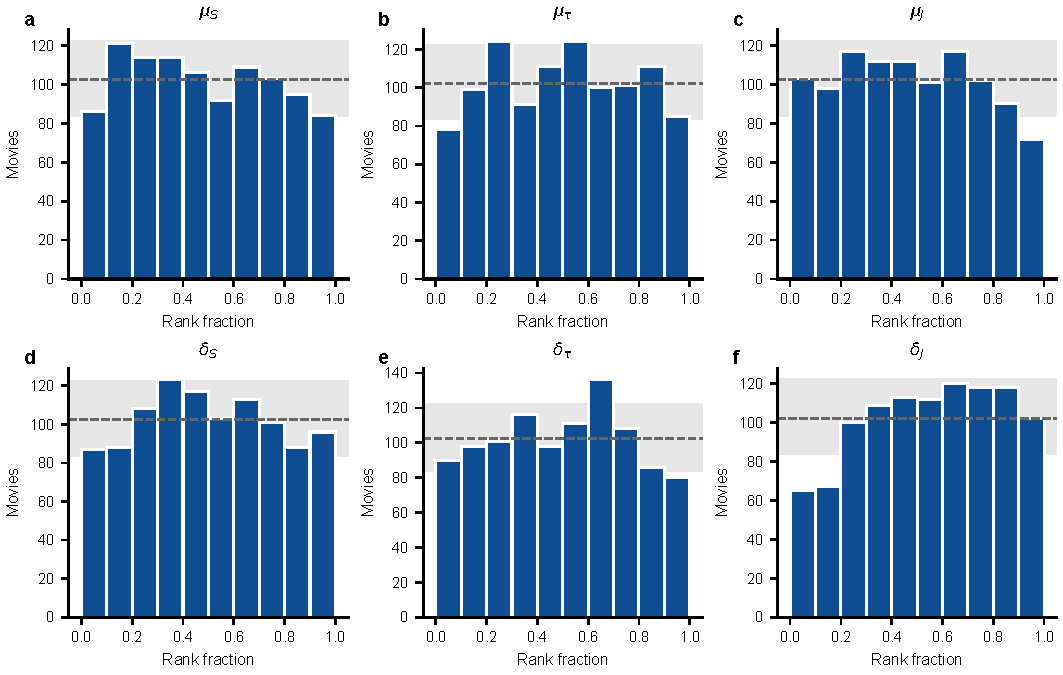
\includegraphics[width=\textwidth]{figures/figS1_rank_calibration.pdf}
\textbf{Marginal posterior-rank diagnostics.} Rank fractions of the generating parameter within the frozen neural posterior are shown for 1,024 independent expanded prior-predictive movies. Gray bands are pointwise 95\% binomial intervals for ten equally sized rank bins; the dashed line gives the expected count. These bands are descriptive and do not provide simultaneous coverage across bins or parameters. A visually uniform histogram does not establish joint or conditional posterior calibration. Source data are provided.

\clearpage
\subsection*{Supplementary Figure S2}
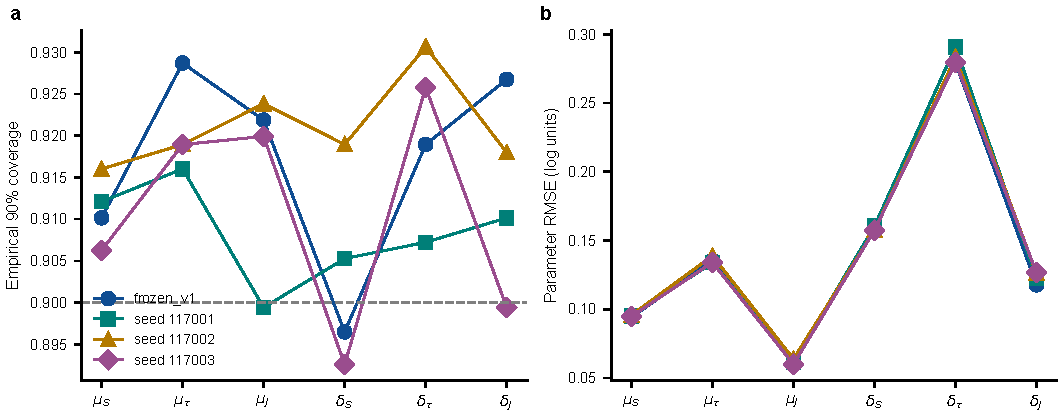
\includegraphics[width=\textwidth]{figures/figS2_training_seeds.pdf}
\textbf{Training-seed sensitivity under the fixed observation design.} \textbf{a}, Nominal 90\% marginal coverage. \textbf{b}, Posterior-median root-mean-squared error. The frozen original network and three new training seeds use a common 16,000-movie bank and are evaluated on the same 1,024 new movies. Connected points identify a model, not repeated measurements that increase the evaluation denominator. New seeds vary initialization, splitting and optimization conditional on the shared bank. Source data are provided.

\clearpage
\subsection*{Supplementary Figure S3}
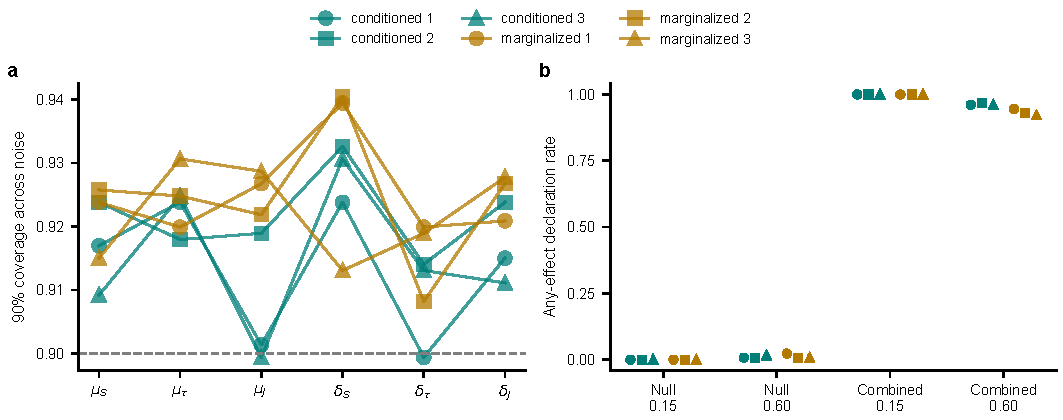
\includegraphics[width=\textwidth]{figures/figS3_noise_training_seeds.pdf}
\textbf{Noise-aware inference across training seeds.} \textbf{a}, Marginal 90\% coverage across 1,024 independent varying-noise movies. \textbf{b}, Any-effect declaration rates for four fixed-noise scenarios, each with 128 independent movies shared across models. Teal denotes conditioning on known noise and ochre denotes marginalizing noise. Marker shape distinguishes three training seeds. The range across seeds is descriptive and is not a confidence interval. Source data are provided.

\clearpage
\subsection*{Supplementary Figure S4}
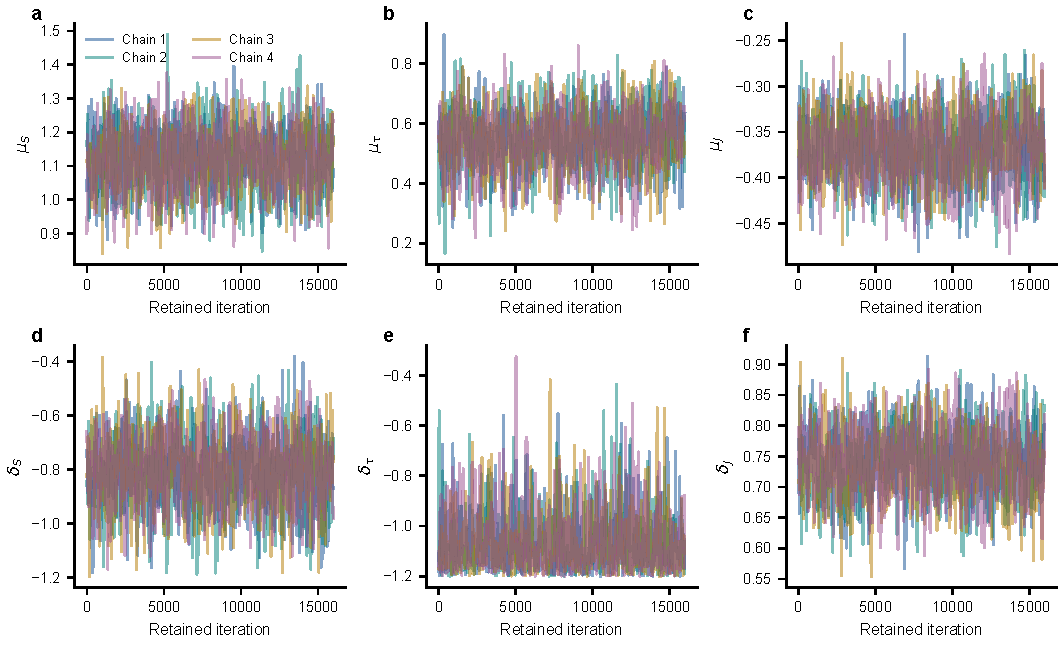
\includegraphics[width=\textwidth]{figures/figS4_sampler_traces.pdf}
\textbf{Posterior sampling for the fixed first combined example.} Four chains are shown for the six global parameters of the prespecified original combined movie. Display thinning reduces file size only; diagnostics and inference use the retained draws without this display thinning. The example was fixed before inspecting recovery accuracy. Its final diagnostic gate passed after additional sampling. This plot illustrates sampling behavior for one movie; expanded ensemble diagnostics are in Supplementary Fig.~S7. Source data are provided.

\clearpage
\subsection*{Supplementary Figure S5}
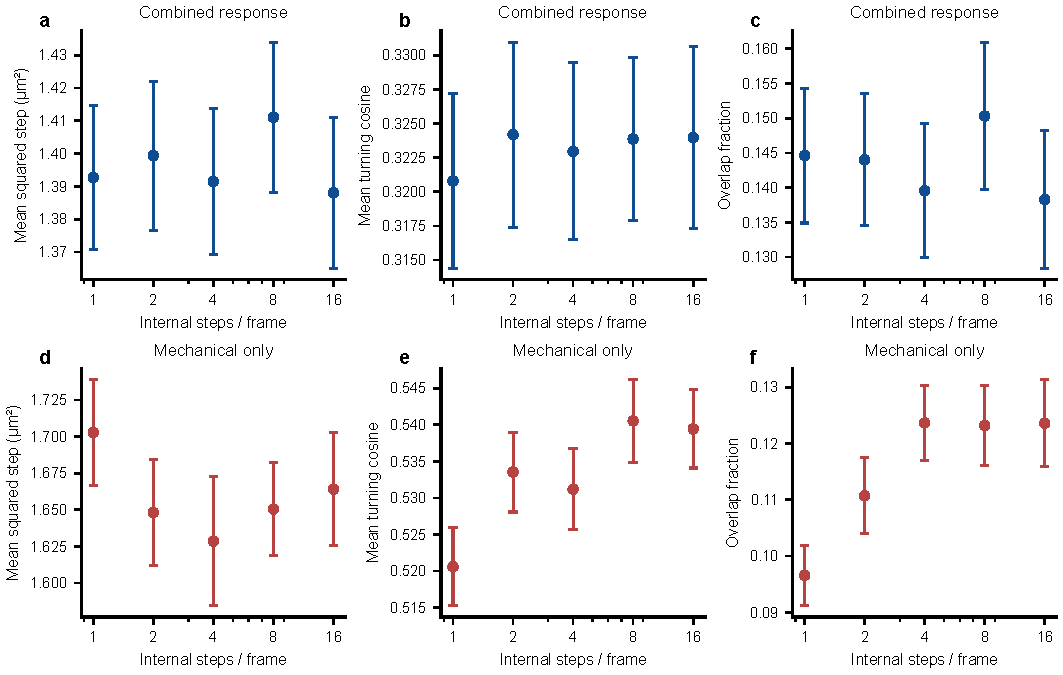
\includegraphics[width=\textwidth]{figures/figS5_timestep.pdf}
\textbf{Weak timestep sensitivity in motion and mechanics.} Mean squared step, turning cosine and overlap fraction are shown for combined motility changes (top) and mechanical-only dynamics (bottom). Each point summarizes 128 independent movies; bars show the mean plus or minus 1.96 Monte Carlo standard errors. Five internal-step settings are evaluated independently, so the figure tests ensemble behavior rather than paired pathwise error. The 16-step setting is a numerical reference, not known exact truth. Source data include the additional exposure and net-displacement metrics.

\clearpage
\subsection*{Supplementary Figure S6}
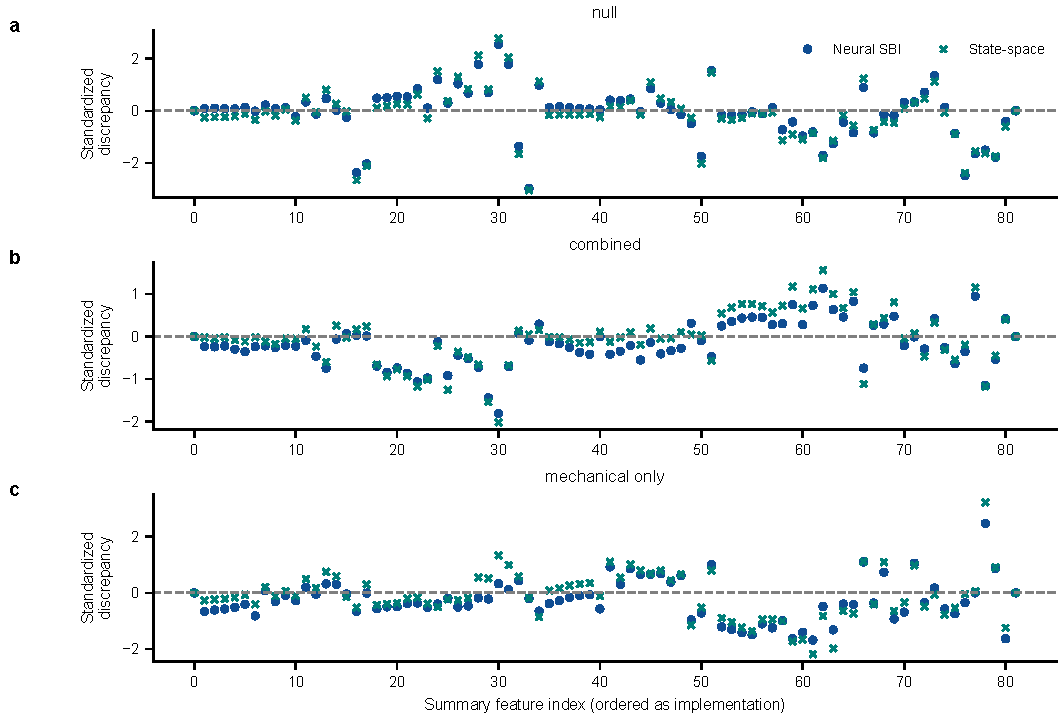
\includegraphics[width=\textwidth]{figures/figS6_predictive_checks.pdf}
\textbf{Selected predictive summaries can miss omitted mechanics.} For the fixed first null, combined and mechanical-only examples, observed summary deviations from the predictive mean are divided by predictive standard deviation. One hundred geometry-conditioned predictive movies per method/example redraw cell offsets. Markers show neural and state-space fitted baseline predictions. Feature order follows the implementation, and exact feature values are supplied as source data. Features are correlated; the standardized discrepancies are not independent tests or an omnibus calibrated diagnostic.

\clearpage
\subsection*{Supplementary Figure S7}
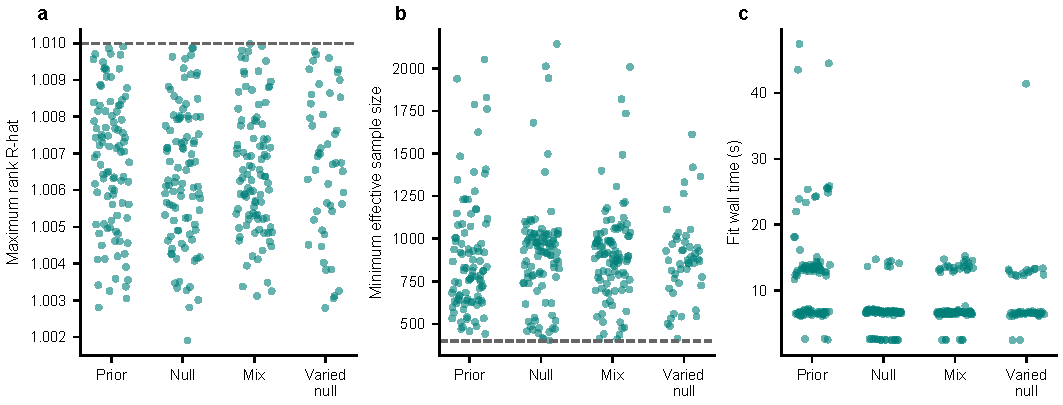
\includegraphics[width=\textwidth]{figures/figS7_numerical_diagnostics.pdf}
\textbf{Expanded state-space numerical checks.} Final maximum rank-normalized $\widehat R$, minimum bulk/tail effective sample size and per-movie elapsed fitting time are shown for the four new ensembles. The thresholds are $\widehat R<1.01$ and effective sample size at least 400 for every global and cell parameter. Elapsed time includes retries and orchestration as recorded; concurrent workers share hardware. Numerical acceptance is distinct from model adequacy. Attempt histories and unresolved counts are retained in source records.

\clearpage
\subsection*{Supplementary Figure S8}
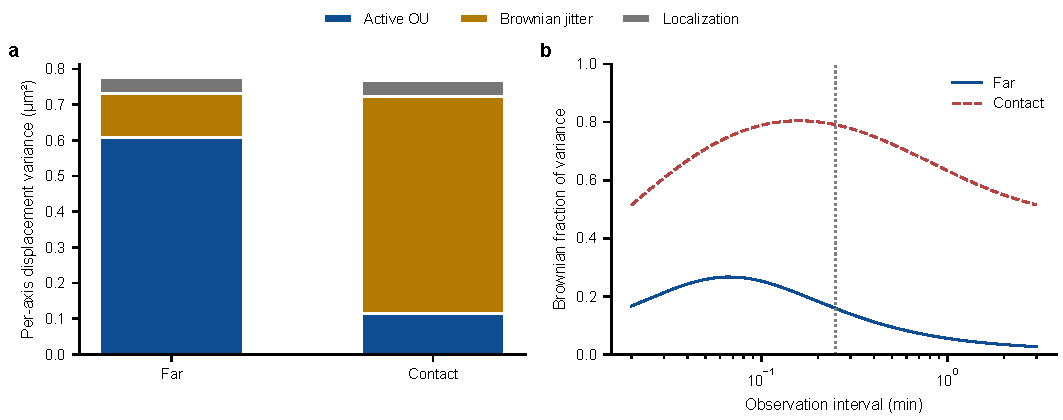
\includegraphics[width=\textwidth]{figures/figS8_local_variance.pdf}
\textbf{An analytical illustration of changing information content.} \textbf{a}, Locally stationary per-axis displacement-variance components far from a target and at contact under the strong combined alternative, for zero cell offset and the 0.25-min recording interval. \textbf{b}, Brownian-jitter fraction of the same local variance over different observation intervals; the dotted line marks 0.25\,min. These curves follow the stated constant-coefficient equations and are not fitted biological measurements or a proof of identifiability. Source data are provided.

\clearpage
\section{Reproduction and outstanding author decisions}
A complete reproduction starts with the core synthetic benchmark, followed by the two manuscript expansion scripts, the publication-figure script and the manuscript builder. The source snapshot provides the exact command sequence and environment versions. Scripts preserve original and follow-up results in different directories. The final manuscript builder reads saved numerical results rather than embedding manually typed estimates, verifies shared-movie hashes and exports a numeric claim ledger.

The manuscript uses a standard \texttt{article} class, default Computer Modern fonts, embedded numerical references, unnumbered Results/Methods subheadings and a separate supplement. It is a journal-style research draft, not an accepted paper or official publisher template. Author and affiliation fields are blank at the user's request. Funding, contributions, competing interests, permanent repositories, license selection and human verification remain to be supplied. No journal submission or public repository release has been performed.
\end{document}
